\section{Sepsis}

Sepsis is a condition that develops on behalf of an infection or bacteria in the tissue within the body which triggers an immune response that overexposures the workload on the immune system to fight the inflammation or bacteria. The infection or bacteria can be anywhere in the body’s tissue. Some of the normal macrohaemodynamics of sepsis are abnormal body temperature, abnormal heart rate, oxygen extraction and abnormal blood pressure \citep{plunta2010}.
...

Under sepsis several things happen in the microcirculatory system that leads to impaired homeostasis in the body, because it’s in the microcirculatory system that is responsible for aiding the tissue with oxygen and nutrients delivery and removal of waste products. In the blood infection or other bacteria that’s responsible for causing some irregularity in the blood is present or in the tissues around the the blood vessels. Among the first thing’s that happens when the body encounters an infection, white blood cells are recruited to release molecules that will fight the infection. Molecules that interact with the endothelia in the blood vessels, like nitric oxide (NO, are released. The interaction causes the blood vessels to dilate to increase the blood vessel diameter and permeability. The increased diameter slows down the blood flow, which causes a drop in blood pressure. Also the vessels permeability is increased. This reaction happens multiple places in the body where there is infected tissue present and will cause systemically vessel dilation.
When the permeability of the blood vessels is increased there will be more fluid in the tissue from the blood and the cells gets less oxygen because the oxygen has a harder time to get to the tissue. Also the blood vessels will get damaged when the white blood cells try to destroy the pathogens. This triggers coagulation and clotting is formed in the damaged areas in the blood vessels, clots can break off into the blood. The damaged blood vessels leads to more leakage because there will be a point where the coagulation can’t follow up \citep{baudouin200}.

Septic shock happens when the body has undergone sepsis for a greater duration of time. When the cells are not getting a sufficient supply of oxygen and therefore the cells will begin to die. This can lead to a very dangerous state, where organs begin to fail because they get damaged. When multiple organs get damaged the state in septic shock reaches multiple organ failure also called multiple organ dysfunction syndrome (MODS). The mortality for patients with septic shock are in the region of 50\% \citep{baudouin200}. 

\begin{figure}[H]
	\centering
	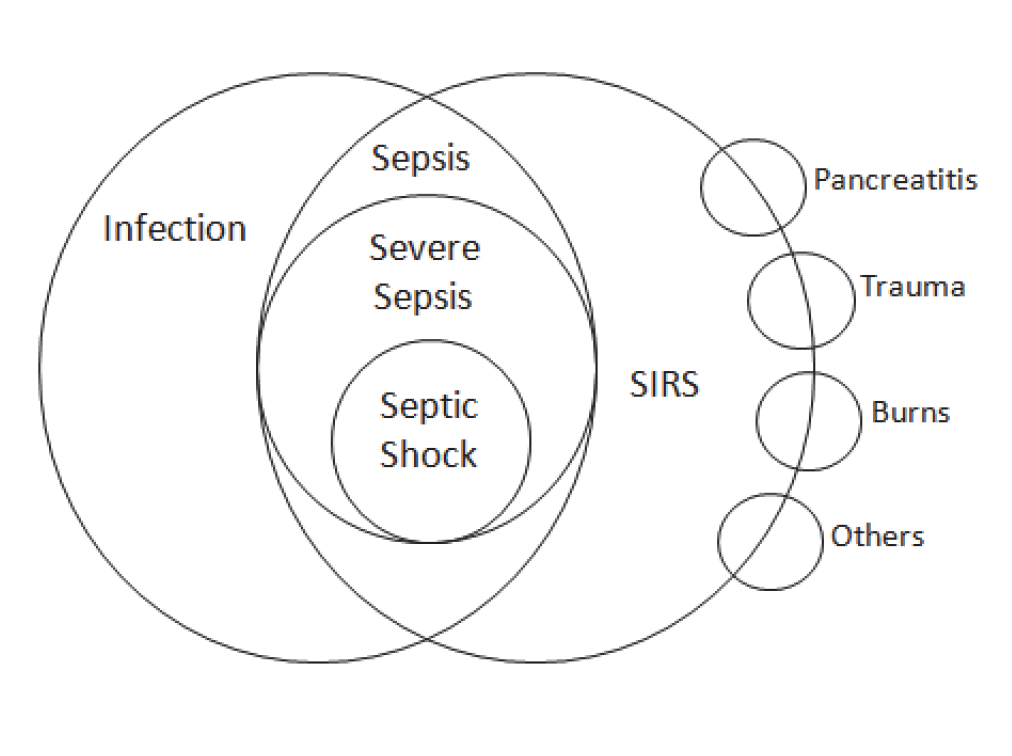
\includegraphics[width=1\textwidth]{figures/Sepsis_stages}
	\caption{Stages in sepsis}
	\label{fig:Sepsis_stages}
\end{figure} \vspace{-.3cm}
